\documentclass[utf8,xcolor=table, page number]{earlywinter}

\usepackage[T1]{fontenc}
\usepackage[frenchb]{babel}
\usepackage{graphicx}

\begin{document}
\title{Edge Cloud Computing}
\subtitle{Bringing the Cloud to the Edge}
\author{Aurèle BARRIÈRE & Solène MIRLIAZ}
\date{05/04/2017}

\begin{frame}[plain]
  \titlepage%
\end{frame}

% ----------------
% - Introduction -
% ----------------
\section*{Introduction}
\begin{frame}
	\frametitle{\secname}
  \framesubtitle{Cloud model}
  \begin{center}
    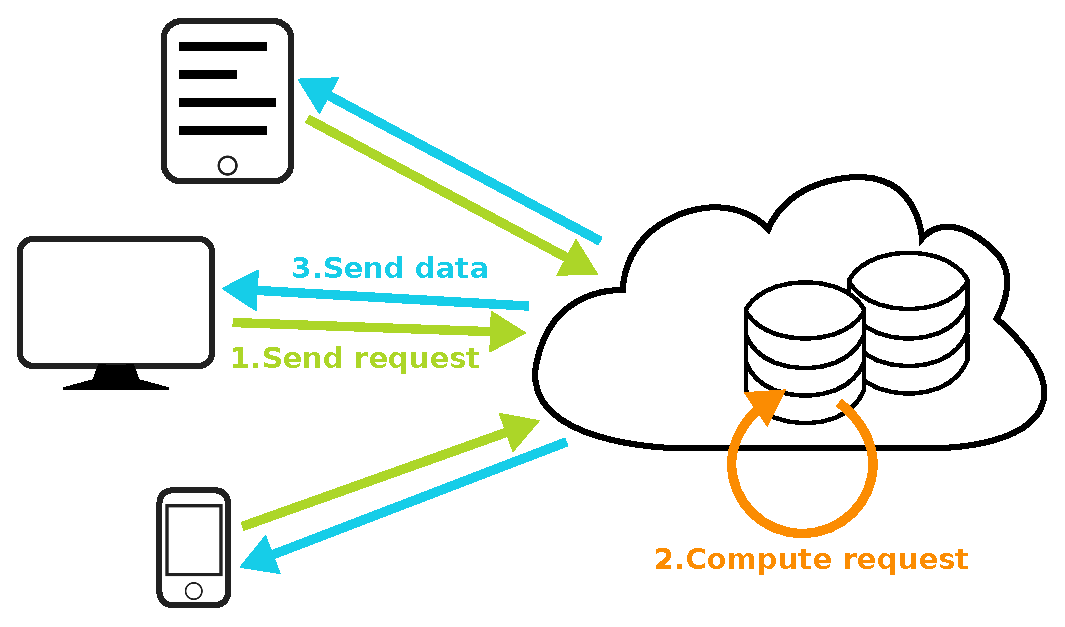
\includegraphics[width=0.7\linewidth]{cloud.eps}
  \end{center}
  \begin{block}{Principle}
    Optimize resource usage
  \end{block}
\end{frame}
\begin{frame}
	\frametitle{\secname}
  \framesubtitle{Cloud limits}
  \begin{minipage}[l]{0.6\linewidth}
  \begin{block}{Internet of things}
    Growth of the number of connected objects and sensors that generate data.
    The end nodes are evolving from consumers to producers.
    
    Estimated produced data by 2019: \emph{500 zettabytes} {\tiny (estimate by Cisco Global Cloud Index)}.
  \end{block}
  \end{minipage}
  \begin{minipage}[l]{0.3\linewidth}
    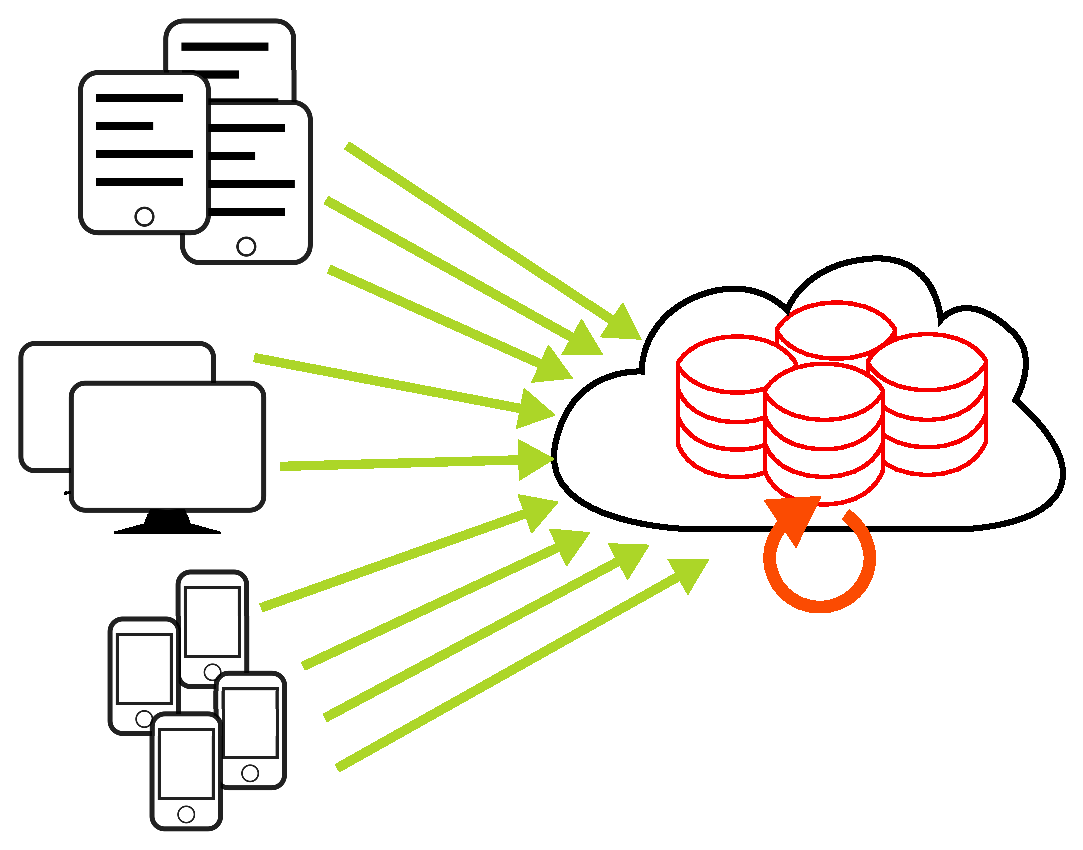
\includegraphics[width=1.5\linewidth]{cloudlimits.eps}
  \end{minipage}
	\begin{alertblock}{Limits of the clouds}
          \begin{itemize}
            \item The network can't handle that much.\\
              Estimated IP traffic by 2019: 10.4 zettabytes.
            \item The Cloud's computation power can't handle that much.
            \item For many uses, the Cloud introduces too much latency.
            \item Centralization brings privacy issues.
          \end{itemize}
	\end{alertblock}
\end{frame}
\begin{frame}
	\frametitle{\secname}
  \framesubtitle{Fog model}
  \begin{center}
    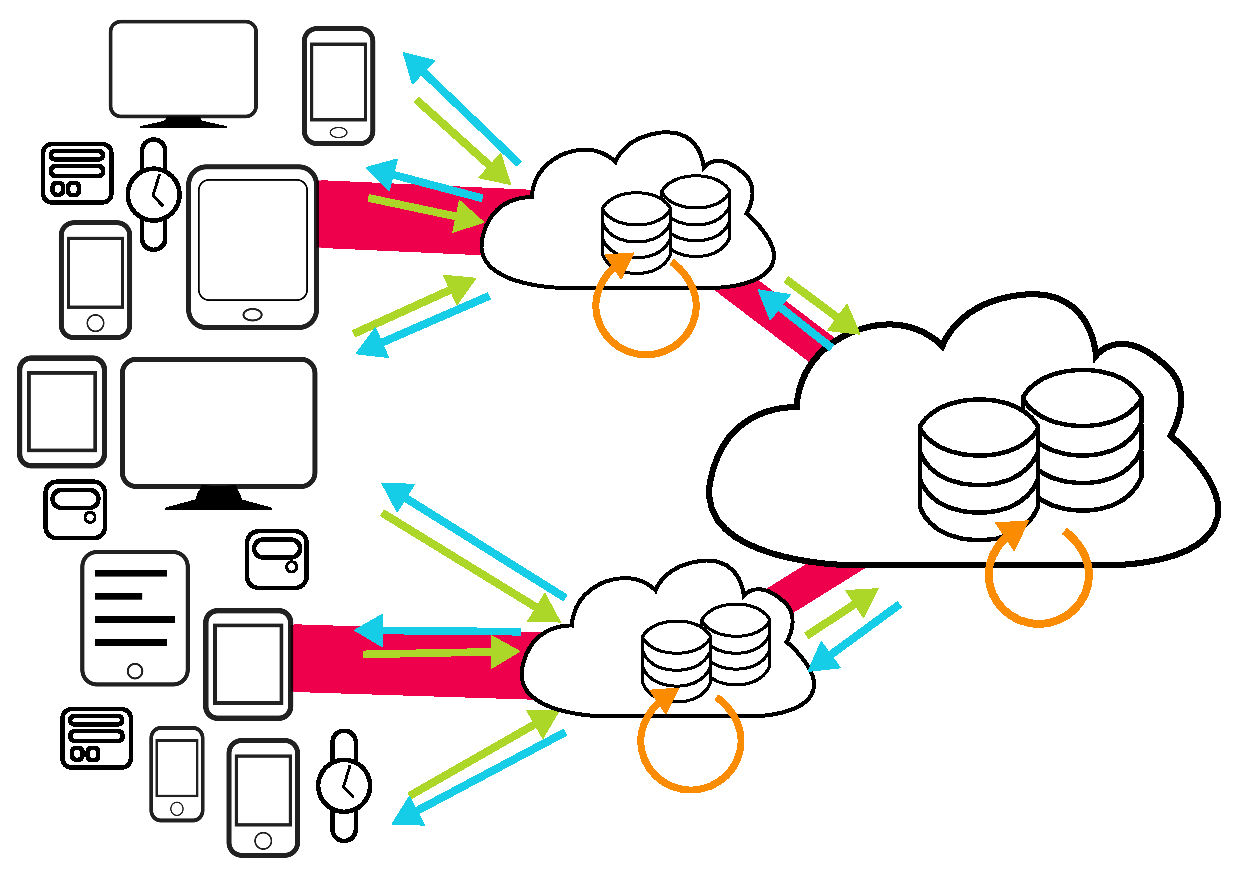
\includegraphics[width=0.6\linewidth]{fog.eps}
  \end{center}
  \begin{block}{Principle}
    More little clouds, closer to the devices $\to$ Spread the resources\\
    Lower latency
  \end{block}
\end{frame}
\begin{frame}
	\frametitle{\secname}
  \framesubtitle{Edge model}
  \begin{center}
    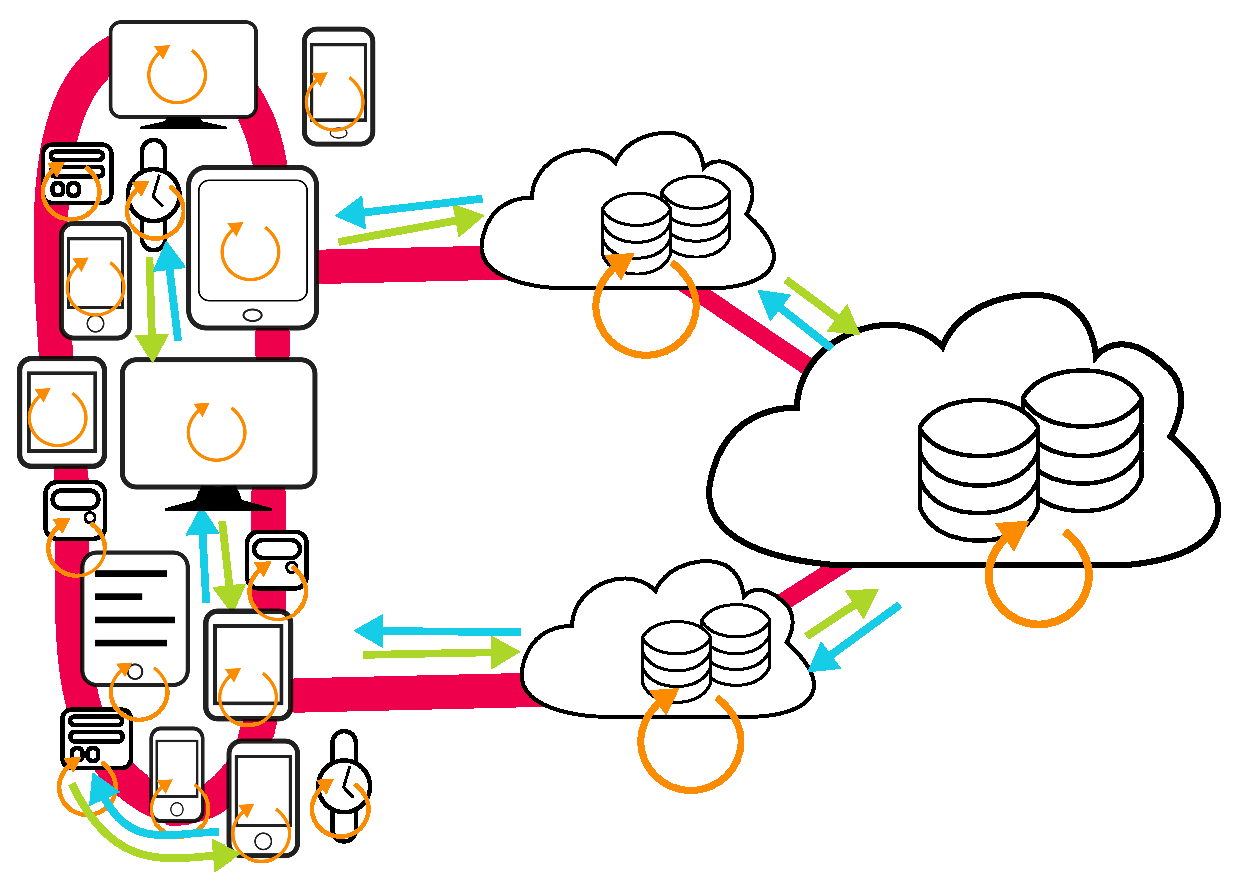
\includegraphics[width=0.6\linewidth]{edge.eps}
  \end{center}
  \begin{block}{Principle}
    More computation done on the devices, more communication between close devices.
  \end{block}
\end{frame}

  \begin{frame}
    \frametitle{Table of contents}
    \tableofcontents[]
  \end{frame}
  
  
\section{Edge computing challenges}
\subsection{Bringing the cloud to the Edge: an hybrid system} %I'm not sure this is a good phrasing. maybe some of the papers we read would disagree
\begin{frame}
  \frametitle{Edge computing}
  \framesubtitle{Principle}

  \begin{block}{Computing in the Edge}
    Increase in the nodes' computing power (smartphones, embedded devices).
  \end{block}
  \vfill
   We want to put computing at the proximity of data sources: at the Edge.

   It could either be in the nodes themselves, or in smaller edge servers. We can use already existing CDNs to put such servers.
  \vfill
   \begin{exampleblock}{Example: Smart Home}
     In a smart home, the data produced by every sensor could be consumed directly without sending it to a data center.
   \end{exampleblock}

\end{frame}

\begin{frame}
  \frametitle{Edge-Cloud computing}
  \framesubtitle{An hybrid system}

%  \begin{figure}
%    \center
%    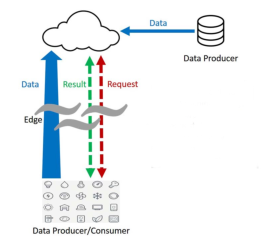
\includegraphics[scale=0.5]{edge.png}  %I'm not a big fan of this graphic. might have to change it.
%  \end{figure}
%
  Keep using the Cloud (core), but add computation at the Edge.
  The Cloud keeps providing global services, but edge servers can compute with lower latency.

  We can then use advantages from both the Cloud and the Edge.
  \vfill
  \begin{exampleblock}{Online Shopping}
    We need a responsive user interface. We want centralized data.\\
    The shopping cart should be located in the edge.\\
    Synchronization with the cloud in the background.
  \end{exampleblock}
  
\end{frame}

\begin{frame}
\frametitle{Edge-Cloud Computing}
\framesubtitle{Overview}

  \begin{center}
    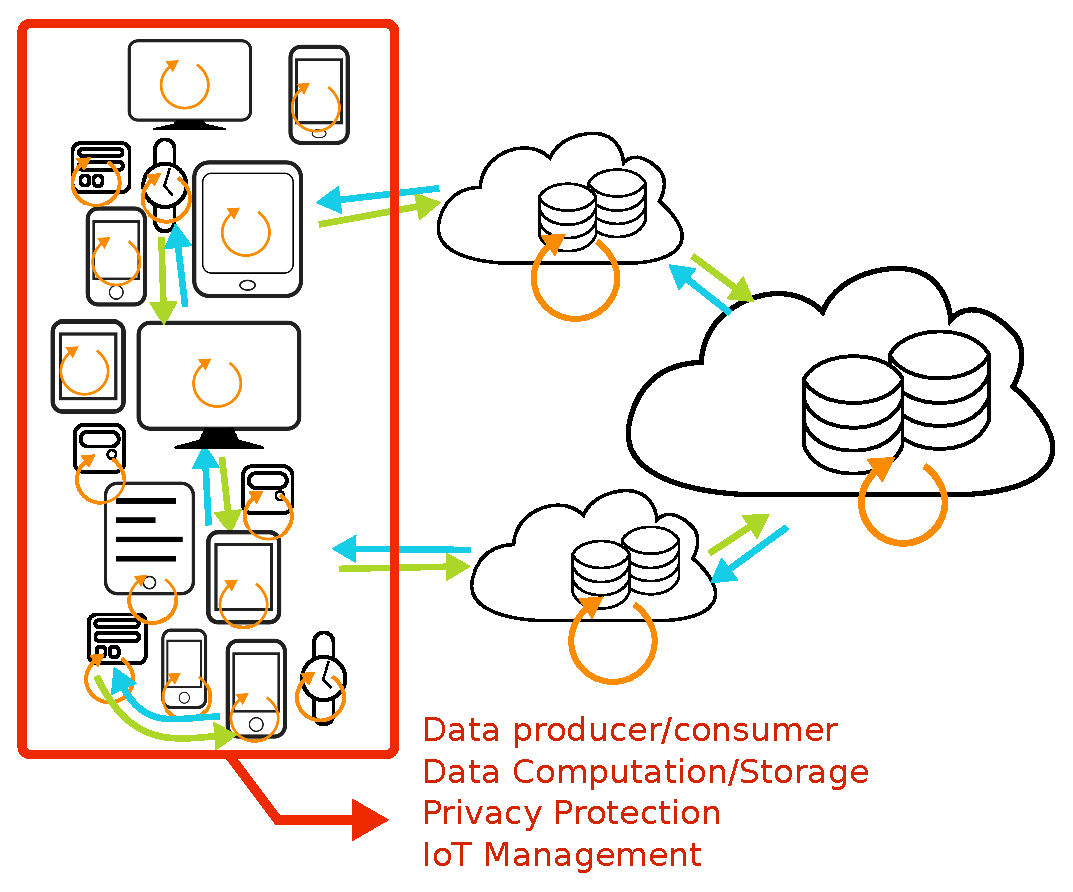
\includegraphics[width=0.6\linewidth]{edgePrinciple.eps}
  \end{center}
  
  \begin{alertblock}{Hybrid System}
    No suppression of the cloud
  \end{alertblock}

\end{frame}

\subsection{Challenges}

% the challenges and research interests are almost the same to me

\begin{frame}
  \frametitle{\subsecname}
  \framesubtitle{Overview}
  \begin{description}
    \item[{\color{orange!95!black}Energy}] Mobile devices have a battery so limited energy\\
      $\neq$ Green computing
    \item[{\color{orange!95!black}Mobility}] Access, availability, etc.\\
      Need a strong failure-tolerance system.\\
      Service localization ?
    \item[{\color{orange!95!black}Heterogeneity}] More than in the cloud.\\
      \begin{itemize}
        \item Devices: from a computer to a connected thermometer\\
        \item Network: High-speed links in data center to wireless communication
        \item Applications: in real-time, lots of communication, lots of computing,
      high memory needs, etc.
      \end{itemize}
  \end{description}
\end{frame}

\begin{frame}
  \frametitle{\subsecname}
  \framesubtitle{Overview}
  \begin{description}
    \item[{\color{orange!95!black}Programmability}] How to deploy an application on different architecture
    \item[{\color{orange!95!black}Naming conventions}] IP Protocols can be heavy for small devices
  \end{description}
\end{frame}

% \section{Current research studies}
% \subsection{Architecture}
% \begin{frame}
%   \frametitle{Current Research}
%   \framesubtitle{Architecture}
% 
%   Edge-cloud computing requires new connections between users, edge nodes, edge networks, datacenters...
% 
%   
% 
% \end{frame}
% \subsection{Workload Distribution}
% \begin{frame}
%   \frametitle{Current Research}
%   \framesubtitle{Workload Distribution}
% \end{frame}
% \subsection{Problem Identification and Heuristics}
% \begin{frame}
%   \frametitle{Current Research}
%   \framesubtitle{Problem Identification and Heuristics}
%   \begin{exampleblock}{On-demand gaming coverage} % [4]
%     We need a low-latency service that can satisfy the most people.\\
%     We need heuristics for edge servers deployment.
%   \end{exampleblock}
% \end{frame}
% \subsection{Programmability}
% \begin{frame}
%   \frametitle{Current Research}
%   \framesubtitle{Programmability}
% \end{frame}
% \subsection{Naming}
% \begin{frame}
%   \frametitle{Current Research}
%   \framesubtitle{Naming}
% \end{frame}
% 
% \section{Case example: a traffic light}
% \begin{frame}
%   \frametitle{Case Example}
%   \framesubtitle{Smart Traffic Light}
% \end{frame}


\section{Use Cases}

\begin{frame}
  \frametitle{Use Cases}
  \framesubtitle{And Research interests}

  \begin{block}{}
    In which cases is Edge-Cloud Computing more efficient than Cloud-only or Edge-only approaches?
  \end{block}

\end{frame}

\subsection{Localization Awareness}
\begin{frame}
  \frametitle{\secname}
  \framesubtitle{\subsecname}

  \begin{exampleblock}{Indoor 3D localization}
    Smartphones gather data from the camera and accelerometer.\\% $\to$ \emph{Data Producer}.\\
    Computation can be done in the edge (latency) or in the core (reliability).
  \end{exampleblock}

  \begin{minipage}[l]{0.3\linewidth}
    \begin{exampleblock}{Computation}
      Computation intensive problem $\to$ needs to be sent to the core
    \end{exampleblock}
  \end{minipage}
  \begin{minipage}[l]{0.65\linewidth}
  \begin{center}
  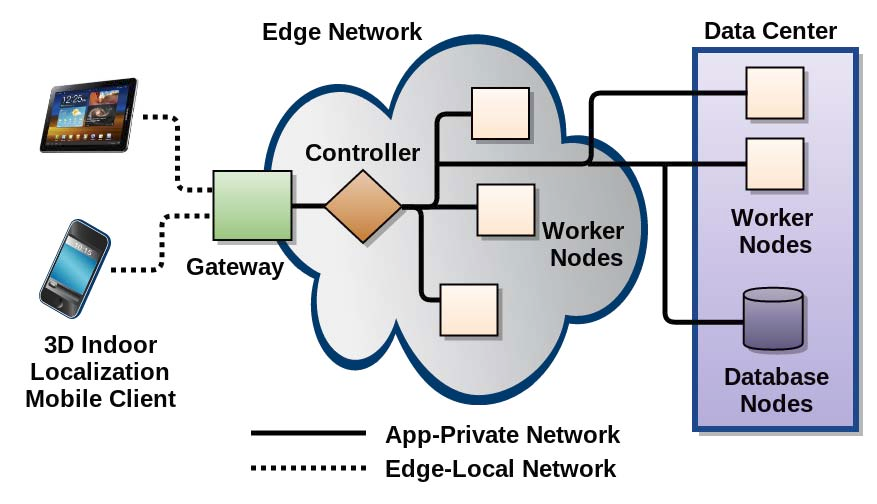
\includegraphics[scale=0.2]{indoor}
  \end{center}
  \end{minipage}

\end{frame}

\subsection{Reducing the network usage}
\begin{frame}
  \frametitle{\secname}
  \framesubtitle{\subsecname}

  \begin{alertblock}{Limit of the network's capacity}
    Internet of Things, increase in produced data.% $\to$ Limit of the network capacity
  \end{alertblock}
  \vfill
  \begin{exampleblock}{Smart Cities, Smart Homes}
    One city in 2019 = 180PB of data per day (health, utility, transports, etc).\\
    Need low latency for health emergency of public safety \\
    Smart home: Cheap sensors in the floors, the walls, electronic devices..\\
    A lot of the produced data could be consumed locally.\\
    We could still use centralization but we can't connect everything to the Cloud.
  \end{exampleblock}
  
\end{frame}


\subsection{Computing at different time scales}
\begin{frame}
  \frametitle{\secname}
  \framesubtitle{\subsecname}

  \begin{exampleblock}{Online Shopping}
    We need a responsive user interface. We want centralized data.\\
    The shopping cart should be located in the edge.\\
    Synchronization in the background.
  \end{exampleblock}
  \vfill
  \begin{exampleblock}{Smart Traffic Light System}
    We want centralized data to regulate traffic on a large scale.\\
    We want low-latency response when dealing with local events.

  \end{exampleblock}
  
%  \begin{block}{Needs}
%    \begin{enumerate}
%      \item real-time, local
%      \item near real-time
%      \item storage of data for later analysis
%    \end{enumerate}
%  \end{block}
%  
\end{frame}


\begin{frame}
  \frametitle{\secname}
  \framesubtitle{\subsecname: Smart Traffic Light system}
  

  \begin{minipage}[l]{0.7\linewidth}
  \begin{block}{Smart Traffic Light}
    Sensors for vehicles and pedestrians.
  \end{block}

  \begin{block}{Goals}
    \begin{itemize}
    \item Accident prevention.
    \item Maintenance of a steady traffic flow.
    \item Data gathering.
    \end{itemize}
  \end{block}
  \end{minipage}
\begin{minipage}[l]{0.2\linewidth}
  \begin{center}
    
\includegraphics[width=0.7\linewidth]{trafficlight.png}
  \end{center}
  \end{minipage}

  \begin{exampleblock}{Two different time scales}
    \begin{itemize}
    \item Prevent collisions: a few milliseconds.
    \item Traffic control: a few seconds or minutes.
    \end{itemize}
  \end{exampleblock}
\end{frame}


\subsection{Reduce the workload in the Cloud}
\begin{frame}
  \frametitle{\secname}
  \framesubtitle{\subsecname}

  \begin{exampleblock}{Video Surveillance}
    Goal: Find a missing child using all filming devices available.\\
    Problem: The huge amount of data cannot be send to the core without latency.\\
    Idea: Preprocess it at the edge.
  \end{exampleblock}
  \vfill
  \begin{alertblock}{Issues}
    When is it better to preprocess than to send?
  \end{alertblock}

\end{frame}

\begin{frame}
  \frametitle{\secname}
  \framesubtitle{\subsecname}
  \begin{alertblock}{Programmability}
    If we want our application to run on nodes, edge servers, could data centers...\\
    We need a suitable API.\\
    Problem: High heterogeneity of the devices
  \end{alertblock}
  \vfill
  \begin{alertblock}{Workload Distribution}
    We are using heterogeneous and mobile resources for computation.\\
    Problem: How to assign the tasks?
  \end{alertblock}
  
\end{frame}


\subsection{Better coverage for low-latency applications}
\begin{frame}
  \frametitle{\secname}
  \framesubtitle{\subsecname}

  \begin{exampleblock}{On-demand Gaming}
    The service needs low-latency.\\
    Cloud servers could only cover less than 75\% of the US population.\\
    Edge only (service placed on CDN) give the same result with 400 edge-sites of five servers.\\
    An hybrid system is needed.
  \end{exampleblock}

  \begin{minipage}[l]{0.45\linewidth}
    \begin{alertblock}{Heuristics for a better coverage}
      We need the most efficient way to put edge servers.\\
      It is a NP-hard problem.
    \end{alertblock}
  \end{minipage}
  \begin{minipage}[l]{0.5\linewidth}
  \begin{center}
  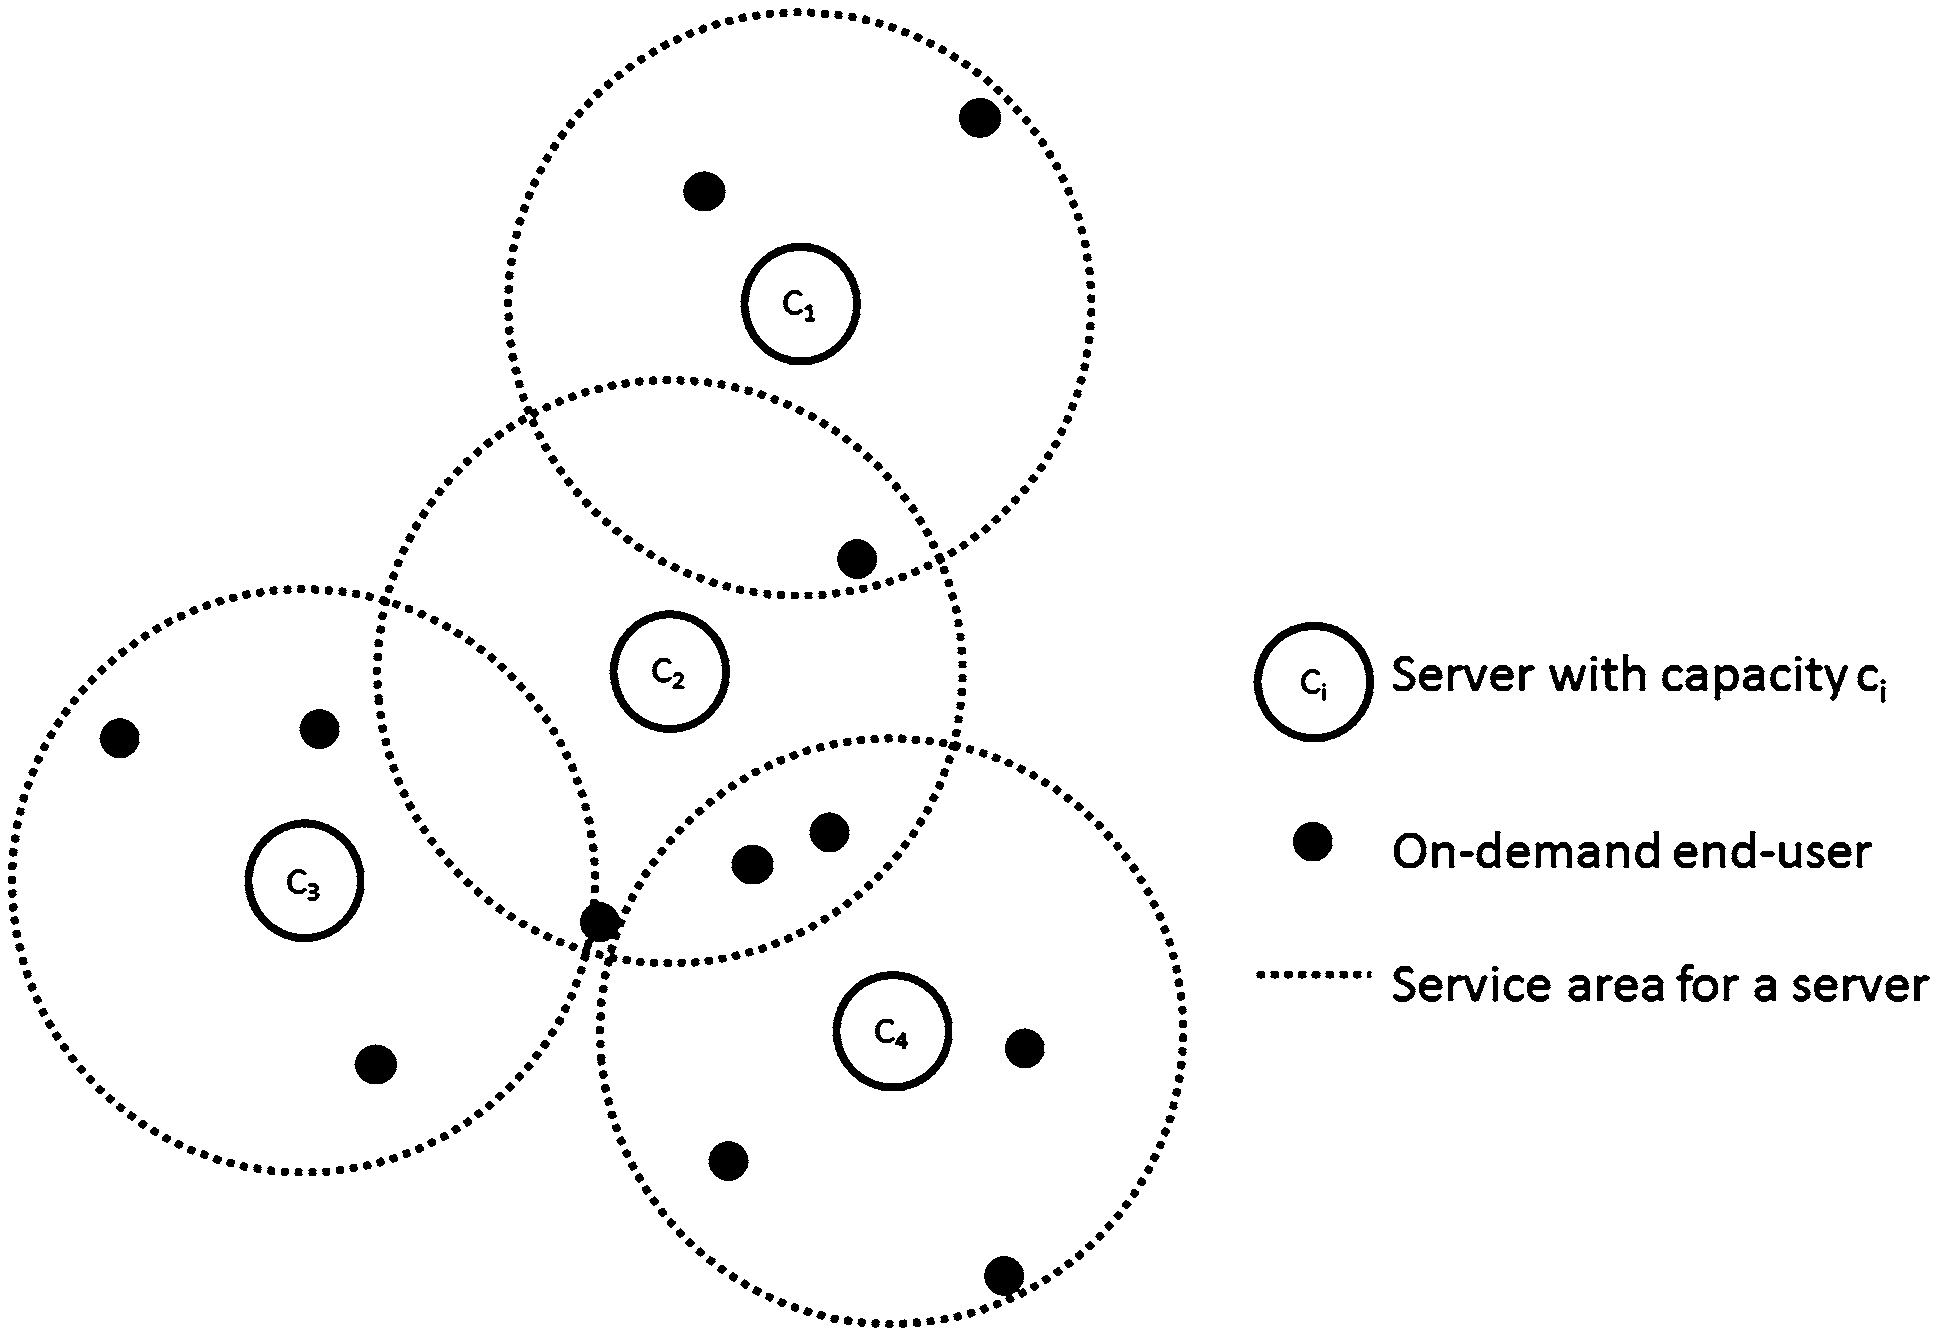
\includegraphics[width=\linewidth]{coverage}
  \end{center}
  \end{minipage}
  
\end{frame}

\begin{frame}
  \frametitle{\secname}
  \framesubtitle{\subsecname}

  \begin{exampleblock}{Heuristics for a better coverage}
    \begin{itemize}
      \item Random: Part of the CDNs are randomly assigned the job of content distribution servers (called smart edges).
      \item Population: The smart edges are spread according to population.
      \item Region: Each geographical region must have at least $x$ smart edges.
      \item Vote for closest latency.
      \item Vote for all: a server vote for the $n$ servers with less than $x$ ms of latency. Weight of the vote is $1/n$.
    \end{itemize}
    Results: Practically no improvement brought by the heuristics compared to the random strategy.
  \end{exampleblock}
  
\end{frame}

\begin{frame}{Other Research studies} % I don't really like this name. any suggestion?
  
  \begin{alertblock}{Privacy}
    Some data cannot be sent to anyone (Electronic Medical Records).
  \end{alertblock}
  \vfill
  \begin{alertblock}{Naming Conventions}
    IP protocol isn't suited for the mobility of end nodes devices.
  \end{alertblock}

  % WARNING: I should read more about these two issues. I don't want to say anything stupid
  
\end{frame}



\section*{Conclusion}

\begin{frame}
  \frametitle{Conclusion}

  \begin{block}{An hybrid system is needed}
    For some applications, neither cloud-only nor edge-only systems are sufficient.
  \end{block}
  \vfill
  \begin{alertblock}{Not a perfect solution}
    In the case of coverage, any reasonable number of edge servers still let some users without service for now.
  \end{alertblock}
  \vfill
  \begin{alertblock}{There's still a lot of work left}
    \begin{itemize}
      \item Lots of open issues.
      \item No economical model.
    \end{itemize}
  \end{alertblock}

  
\end{frame}


\begin{frame}{When should we use Edge-Cloud Computing?}
% where should we put this?
\begin{itemize}
\item When we need centralized data and low latency (online shopping)
\item When communication from the edge to the core is the bottleneck (Fast video analysis, smart home, smart city)
\item When we can reduce the time of computation by spreading it on the Edge (Video surveillance, missing child)
\item When locality is involved (wind farm, smart city)
\item When some data cannot be shared publicly (hospitals)
\item When some data needs to be stored locally (3D indoor localization)
\item When we want a better coverage for low-latency services (on-demand gaming and multimedia)
\item When we need to analyze data at different time scales (Smart Traffic Light System, wind farm). 
\end{itemize}
\end{frame}


\section{Bibliography}
\begin{frame}{Bibliography}
  \tiny
  \nocite{*}
  \bibliographystyle{apalike}
  \bibliography{../bib/edge.bib}
\end{frame}



\end{document}
